\title{Improving Wireless Internet Access in a Campus Environment}
\author{
        Christopher Desnoyers\\
        cjdesno@mit.edu
            \and
        Tristan Honscheid\\
        tristanh@mit.edu
            \and
        Robert Rusch\\
        rusch@mit.edu
}
\date{\today}

\documentclass[11pt,twocolumn]{article}

\usepackage{graphicx}

\begin{document}
\maketitle

\section{Introduction}
\subsection{Problem}
\indent Campus Wi-Fi networks are cruitical to the operation of a modern univeristy. Such networks may be required to serve tens of thousands of users
through several thousand access points, with high expectations of scalability, reliability, and availability. Despite this, existing 
implementations of 802.11, commonly referred to as Wi-Fi, lack many features that may aid in the smooth operation of such large-scale networks in dynamic 
environments such as a college campus. It is difficult to scale, monitor, and intelligently handle network congestion.
\subsection{802.033}
\indent We seek to propse a new wireless network infrastructure, called 802.033, that implements many features of interest to large network operators.
\subsubsection{Brief System Overview}
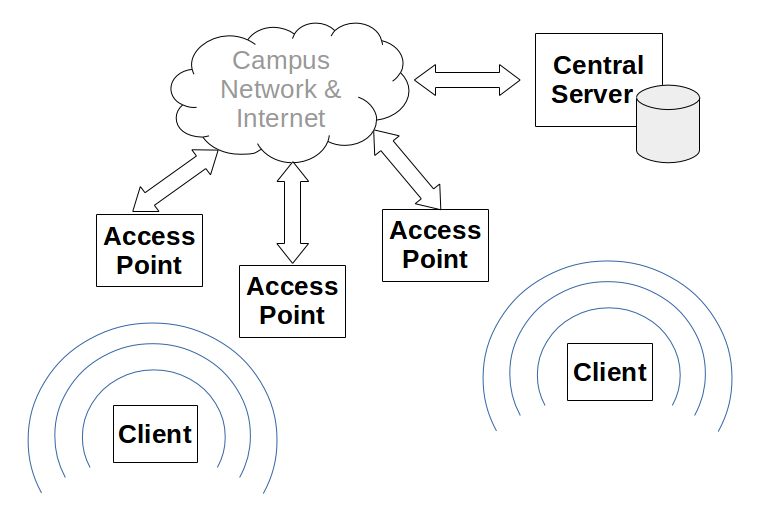
\includegraphics[width=0.5\textwidth]{overview}
\indent The system consists of three main components\\
\begin{enumerate}
	\item \textbf{Central Server:} A central server on the network is used a hub for monitoring of network status information. The server also knows
		the locations and network addresses of each Access Point in the system.
	\item \textbf{Access Points:} Access Points are radio-enabled networked devices capable of connecting Clients to the network. They are
		able to execute customized software for handling connections and congestion.
	\item \textbf{Clients:} The Client is the software on the end-user's device that communicates wirelessly to the network and sends connection information and
		user data to Access Points. The Client is able to determine and communicate the user's bandwidth requirement.
\end{enumerate}
\indent Our system provides the following improvements:\\
\subsubsection{Enhanced Monitoring and Diagnostics}
\indent Because campus networks are large both in terms of users and geographic coverage, maintenance, monitoring, and diagnostics can quickly become a
difficult task. Our system seeks to ease such burdens by incorporating an automatic monitoring system that reports detailed statistics to a central
server for archiving. Such statistics include data on Access Point (AP) utilization, user transfers to other AP's, and user (dis)satisfaction reports.
\indent Such data allows network operators to diagnose or troubleshoot issues. In the long term, it also allows them to discover and forecast trends that
identify areas of insufficient coverage or high user disatisfaction. Analysis of this data can guide the installation of future Access Points.
\subsubsection{Congestion Management}
\indent To enhance network utilization and user happiness, our wireless network performs congestion management to 
\subsubsection{Scalability}
\indent Our system is designed to be scalable. This goal has been achieved by concentrating most of the network's intelligence at the Access Point
level. Because the number of Access Points grows with the size of the network, the network's processing demands should not be able to exceed any
limits. \\
\indent As little functionality as possible has been implemented in the Central Server. The Central Server serves only occasional Access Point lookups (to
find neighboring Access Points, for example) and as a place to store monitoring data. Because there is only one Central Server, this does prevent the 
system from scaling arbitrarily large, but should not be an issue in any reasonably-sized network. 
\end{document}